\section{Theoretical Foundations} \label{sec:theoretical-foundations}
This section gives a brief insight into the mathematical and experimental foundations regarding electron holography, interference gating and time-discrete signals.
\subsection{Electron Holography} \label{ssec:electron-holography}
Placing the investigated object such that it is illuminated by a plane electron wave results in a modulation of both the amplitude $a_{obj}\left(\vb{r}\right)$ and the phase ${\varphi}_{obj}\left(\vb{r}\right)$ effecting the object wave ${\psi}_{obj}\left(\vb{r}\right)$ \cite{Lehmann2002,Lichte2007}:
\begin{equation}
	{\psi}_{obj}\left(\vb{r}\right) = a_{obj}\left(\vb{r}\right) e^{i{\varphi}_{obj}\left(\vb{r}\right)}.
\end{equation}
The corresponding wave length\footnote{The wavelength $\lambda = h/p$ of a particle, with its momentum $p$ and the Planck constant $h$, was introduced by Louis de Broglie in 1924 \cite{BrogliePhD1924}.} of the electrons (for an acceleration voltage of $U_a = \SI{300}{\kilo\volt}$ the wave length is $\lambda = \SI{1.97}{\pico\metre}$), which is notably smaller than the atomic structure of the illuminated object, makes this technique a viable microscopy method \cite{Lichte2007,Gabor1948}. In order to realize electron holography, an unmodulated reference wave ${\psi}_{ref}\left(\vb{r}\right)$ needs to propagate through a vacuum region near the illuminated object \cite{Lehmann2002,Lichte2007}. The desired hologram can then be obtained by coherently superimposing both waves, which is achieved by deflecting them with a so called \emph{Möllenstedt biprism} towards each other under an angle $\beta$ (\cref{fig:EH-setup}) \cite{Moellenstedt1956}. The resulting electron hologram $I_{hol}\left(\vb{r}\right)$ (\cref{fig:EH}) follows as \cite{Lehmann2002,Lichte2007}:
\begin{equation}
	I_{hol}\left(\vb{r}\right) = 1 + a^2\left(\vb{r}\right) + 2\mu a\left(\vb{r}\right)\cos(2\pi \vb{q}_c\vb{r} + \varphi\left(\vb{r}\right) + \theta\left(\vb{r},\vb{q}_c\right))
\end{equation}
where $a\left(\vb{r}\right)$ and $\varphi\left(\vb{r}\right) = {\varphi}_{obj}\left(\vb{r}\right) - {\varphi}_{ref}\left(\vb{r}\right)$ are the amplitude and the phase of the reconstructed image wave ${\psi}_{rec}\left(\vb{r}\right)$, $\abs{\vb{q}_c} = {\beta}/{\lambda}$ is the carrier frequency of the interference fringes, $\mu$ is the corresponding contrast \cite{Lehmann2002,Lichte2007} and $\theta\left(\vb{r}, \vb{q}_c\right)$ is an additional phase modulation \cite{LehmannPhD1997}. This yields the important conclusion that the amplitude $a\left(\vb{r}\right)$ results in a contrast modulation (\cref{fig:EH-AMP}) and the phase $\varphi\left(\vb{r}\right)$ in a bending of the interference fringes (\cref{fig:EH-PH}) \cite{Lehmann2002,Lichte2007}.
\begin{figure}[H]
\captionsetup{belowskip=0pt}
	\centering
	\begin{subfigure}[c]{\textwidth}
		\centering
		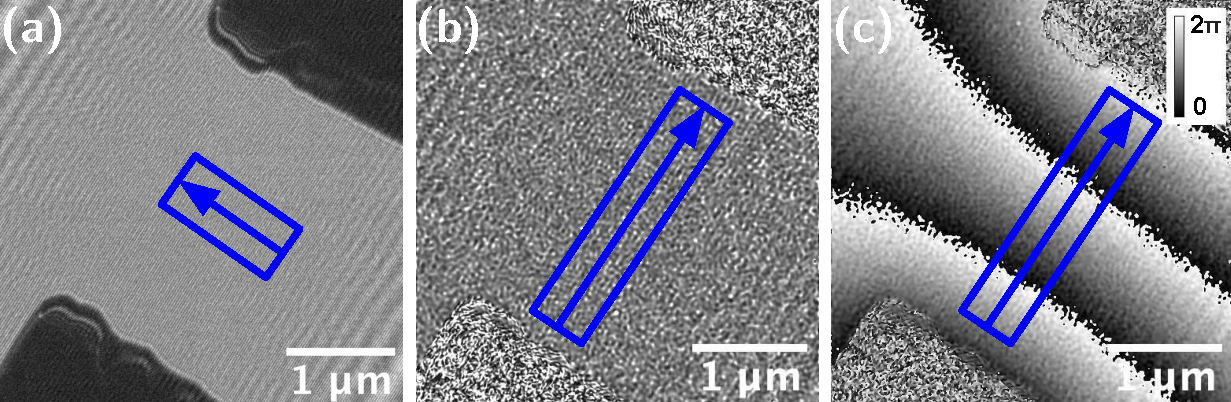
\includegraphics[width=\textwidth]{Figures/Holograms/Holograms.pdf}
	\end{subfigure}
	\hspace{-4mm}
	\begin{subfigure}[c]{0.3\textwidth}
		\centering
		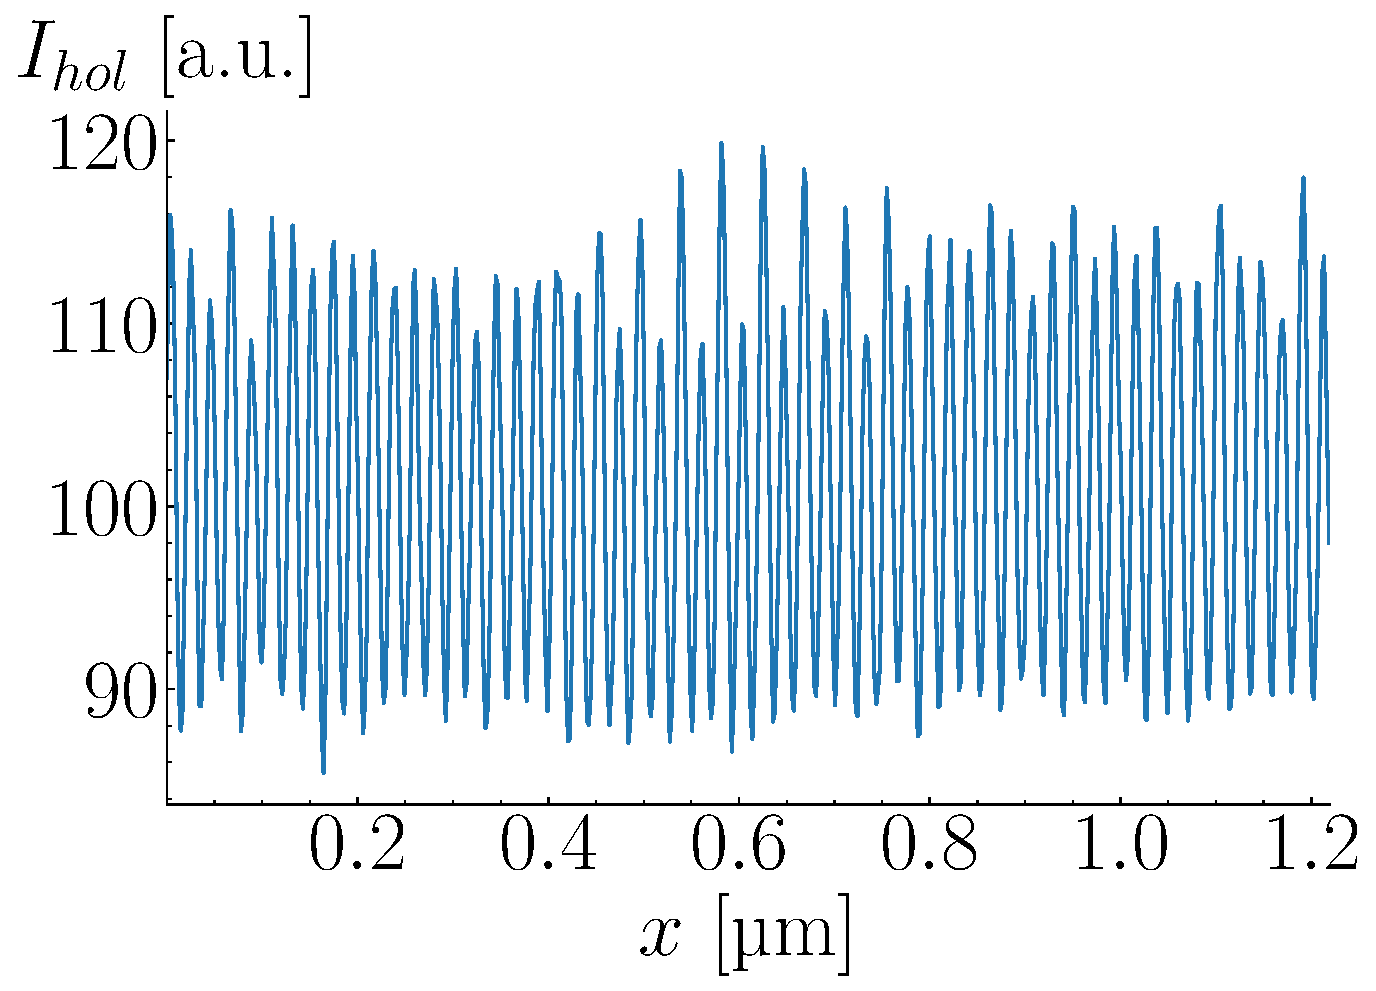
\includegraphics[width=\textwidth]{Figures/Holograms/EH.pdf}
		\phantomsubcaption
		\label{fig:EH}
	\end{subfigure}%
	\hspace{5mm}
	\begin{subfigure}[c]{0.3\textwidth}
		\centering
		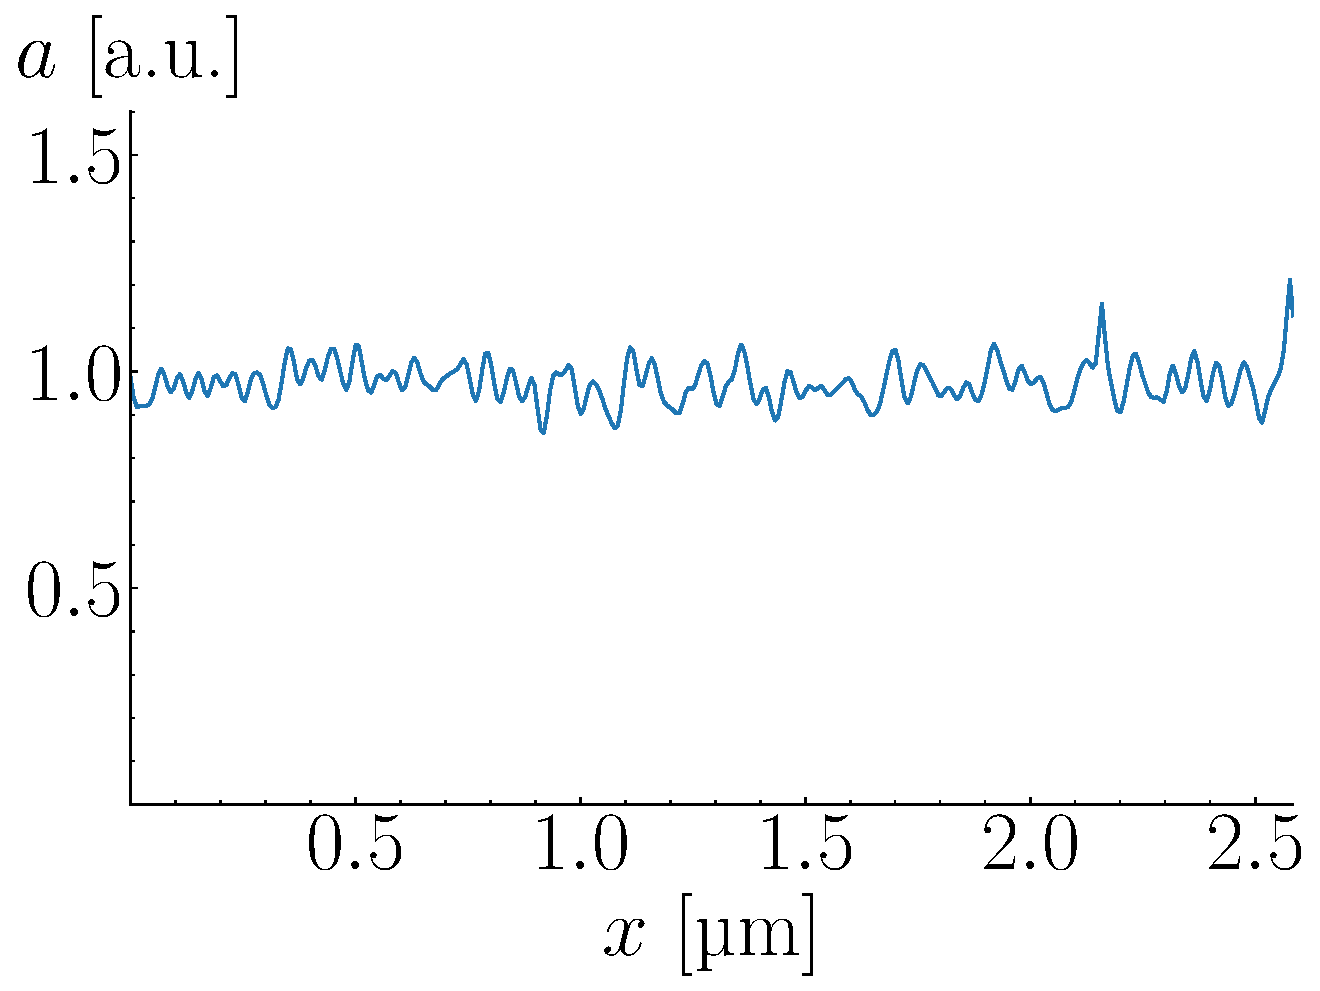
\includegraphics[width=\textwidth]{Figures/Holograms/EH_AMP.pdf}
		\phantomsubcaption
		\label{fig:EH-AMP}
	\end{subfigure}%
	\hspace{4mm}
	\begin{subfigure}[c]{0.3\textwidth}
		\centering
		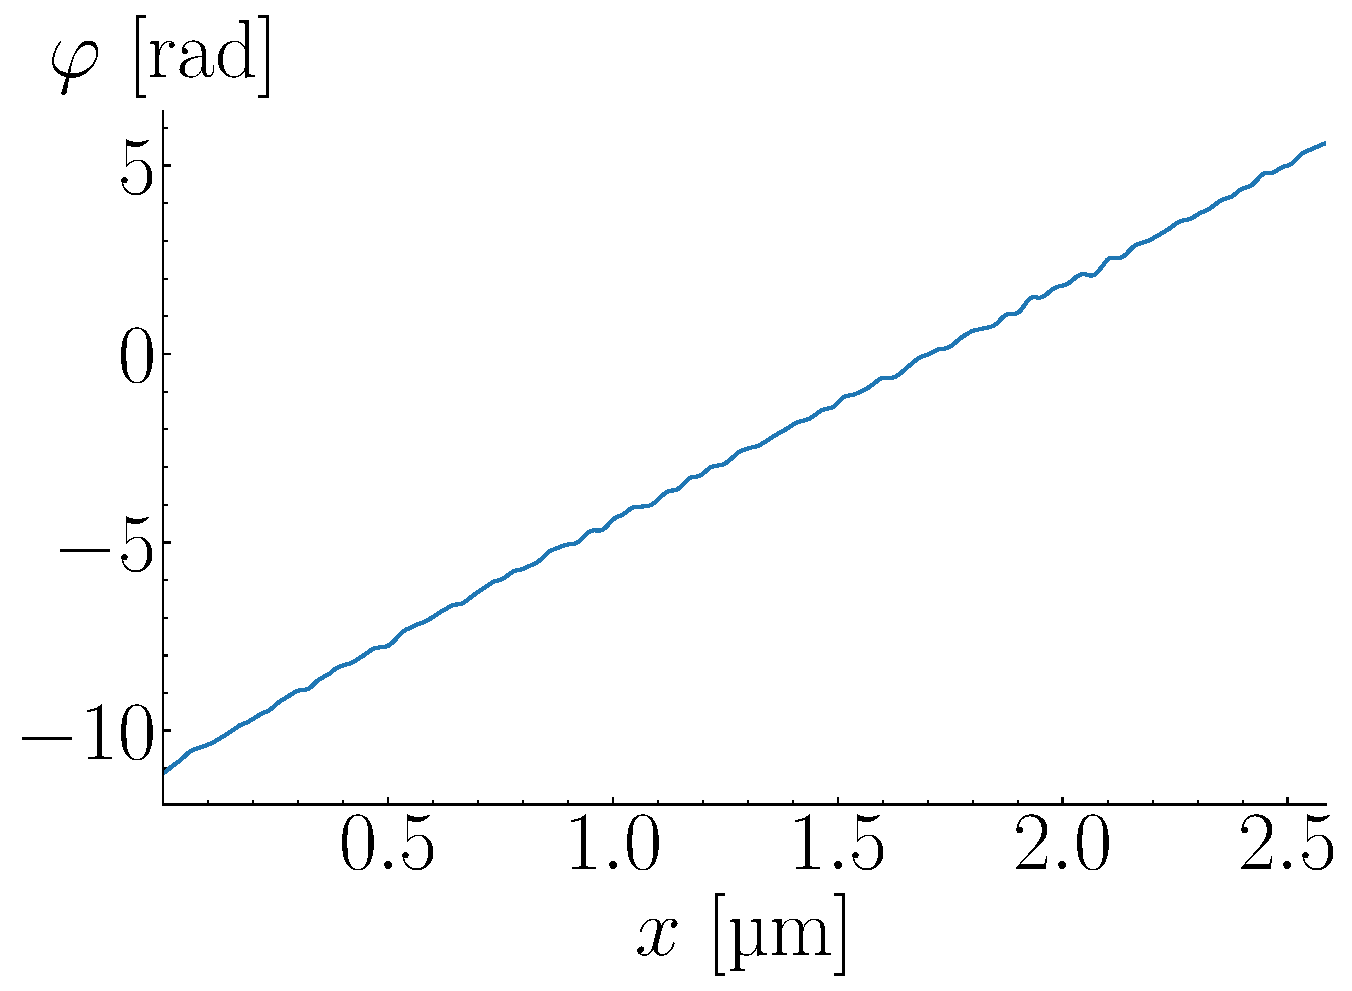
\includegraphics[width=\textwidth]{Figures/Holograms/EH_PH.pdf}
		\phantomsubcaption
		\label{fig:EH-PH}
	\end{subfigure}%
	\caption{Electron holography for a coplanar capacitor biased with $U_{ext} = \SI{1}{\volt}$ with the (a) hologram and its corresponding intensity profile $I_{hol}\left(\vb{r}\right)$, (b) reconstructed amplitude and its corresponding profile $a\left(\vb{r}\right)$ and (c) reconstructed phase and its corresponding unwrapped profile $\varphi\left(\vb{r}\right)$.}
	\label{fig:EH-biased}
\end{figure}
A subsequent Fourier transform of the electron hologram $I_{hol}\left(\vb{r}\right)$ yields \cite{Lehmann1994,Voelkl1995}:
\begin{equation}
	\label{eq:FT-bands}
	\begin{split}
		\mathcal{F}\left\{ I_{hol}\left(\vb{r}\right) \right\} &= \mathcal{F}\left\{ 1 + a^2\left(\vb{r}\right) \right\} \\
		&+ \mu \mathcal{F}\left\{ a\left(\vb{r}\right)e^{i\left(\varphi\left(\vb{r}\right) + \theta\left(\vb{r},\vb{q}_c\right)\right)} \right\} \otimes \delta\left(\vb{q} - \vb{q}_c\right) \\
		&+ \mu \mathcal{F}\left\{ a\left(\vb{r}\right)e^{-i\left(\varphi\left(\vb{r}\right) + \theta\left(\vb{r},\vb{q}_c\right)\right)}\right\} \otimes \delta\left(\vb{q} + \vb{q}_c\right)
	\end{split}
\end{equation}
where the first line of \cref{eq:FT-bands} represents the centerband, the second line the sideband $\left(+1\right)$ and the third line the sideband $\left(-1\right)$ \cite{Lehmann1994,Voelkl1995}. Centering and isolating one of the sidebands in Fourier space allows for the application of an inverse Fourier transform $\mathcal{F}^{-1}$, which in turn leads to the reconstructed image wave ${\psi}_{rec}\left(\vb{r}\right)$ \cite{Lehmann1994,Voelkl1995}:
\begin{equation}
	{\psi}_{rec}\left(\vb{r}\right) = \mu a\left(\vb{r}\right)e^{i\varphi\left(\vb{r}\right)}.
\end{equation}
In order to correct for the various different distortions causing a phase modulation $\theta\left(\vb{r},\vb{q}_c\right)$, an empty hologram is recorded along with every captured object and subtracted from the image phase \cite{voelkl1999,Lichte2007}. Taking the empty hologram $I_{emp}\left(\vb{r}\right)$ immediately after the object holograph results in \cite{voelkl1999}:
\begin{equation}
	I_{emp}\left(\vb{r}\right) = 1 + 2\mu \cos(2\pi \vb{q}_c \vb{r} + \theta\left(\vb{r}, \vb{q}_c\right)).
\end{equation}
If an external bias $U_{ext}$ is applied to the investigated object, therefore modifying its electric potential distribution, a hologram of the unbiased object (i.\,e. $U_{ext} = \SI{0}{\volt}$) can be used as an empty hologram \cite{Niermann2017,Wagner2019}. In doing so, the amplitude $a\left(\vb{r}\right)$ of the reconstructed image wave ${\psi}_{rec}\left(\vb{r}\right)$ is normalized and unwanted phase modulations (e.\,g. induced by surface charging) are automatically subtracted \cite{Wagner2019}.

As an interferometric method, electron holography is susceptible to external disturbances (e.\,g. mechanical vibrations or electromagnetic field fluctuations), requiring a long exposure time of several seconds \cite{Niermann2017}. This limitation imposes special requirements on the coherence properties of the electron source, which has so far limited electron holography to static measurements \cite{Niermann2017}.%
\begin{figure}[H]
	\centering
	\begin{tikzpicture}
	\contourlength{1.5pt}

	\def\centerarc[#1](#2)(#3:#4:#5)[#6][#7]
    {\draw[#1] ($(#2)+({#5*cos(#3)},{#5*sin(#3)})$) arc (#3:#4:#5) node[align=center][#6]{\contour{white}{#7}};}

	\node[rectangle,fill=black!50,draw=black,minimum height=0.75cm,minimum width=0.5cm] (R1) at (0,0) {};
	\node[isosceles triangle,anchor=apex,isosceles triangle apex angle=90,draw=none,rotate=90,fill=black!10,minimum width=3cm] (T1) at (R1.south) {};
	\node[rectangle,fill=black!10,draw=none,minimum height=3cm, minimum width=3cm,anchor=north west] (R2) at (T1.left corner) {};
	\filldraw[fill=black!40,draw=none] (R2.south west) -- (R2.south) -- ++(0,-1.5) -- cycle;
	\filldraw[fill=black!10,draw=none] (R2.south east) -- (R2.south) -- ++(0,-1.5) -- cycle;
	\filldraw[fill=black!30,draw=none] (R2.south west) rectangle (R2.center) node [midway] {${\psi}_{obj}\left(\vb{r}\right)$};
	\filldraw[fill=black!10,draw=none] (R2.center) rectangle (R2.north east) node [midway] {${\psi}_{ref}\left(\vb{r}\right)$};
	\node[rectangle,fill=black!50,draw=black,minimum height=0.2cm,minimum width=1.5cm,ultra thick,anchor=west] (O1) at (R2.west) {};
	\filldraw[fill=black!10,draw=none] ($ (R2.south) + (0,-1.5) $) -- ++(-1,-0.75) -- ++(-0.5,-1.5) -- cycle;
	\filldraw[fill=black!40,draw=none] ($ (R2.south) + (0,-1.5) $) -- ++(1,-0.75) -- ++(0.5,-1.5) -- cycle;
	\filldraw[fill=black!30,draw=none] ($ (R2.south) + (0,-1.5) $) -- ++(-1.5,-2.25) -- ++(3,0) -- cycle;
	\draw[dashdotted] (R1.south) -- ($ (R2.south) + (0,-3.75) $);
	\node[ellipse,fill=black!20,draw=black,minimum height=0.2cm,minimum width=3.5cm,inner sep=0] (E1) at (T1.lower side) {};
	\node[ellipse,fill=black!20,draw=black,minimum height=0.4cm,minimum width=4cm,inner sep=0] (E2) at (R2.south) {};
	\filldraw[fill=black!10,draw=black] ($ (R2.south) + (0,-2.25) $) circle (3pt);
	\node[rectangle,fill=black!50,draw=black,minimum width=0.2cm, minimum height=1cm] (B1) at ($ (R2.south) + (-1.5,-2.25) $) {};
	\node[rectangle,fill=black!50,draw=black,minimum width=0.2cm, minimum height=1cm] (B2) at ($ (R2.south) + (1.5,-2.25) $) {};
	\draw ($ (R2.south) + (-2.5,-3.75) $) -- ++(5,0);
	\node[inner sep=0,align=center,anchor=east] (l1) at ($ (R2.south) + (-2.75,-3.75) $) {Detector};
	\node[inner sep=0,align=center,anchor=east] (l2) at ($ (B1.west) + (-1,0) $) {Biprism};
	\node[inner sep=0,align=center,anchor=east] (l3) at ($ (R2.south) + (-2,-1) $) {Back Focal\\Plane};
	\node[inner sep=0,align=center,anchor=east] (l4) at ($ (E2.west) + (-1,0) $) {Objective};
	\node[inner sep=0,align=center,anchor=east] (l5) at ($ (E1.west) + (-1,0) $) {Condenser};
	\node[inner sep=0,align=center,anchor=east] (l6) at ($ (O1.west) + (-1,0) $) {Object};
	\node[inner sep=0,align=center,anchor=east] (l7) at ($ (R1.west) + (-1,0) $) {Electron\\Source};
	\draw[bend right=30] (l3.east) to ($ (R2.south) + (0,-1.5) $);
	\draw (l2.east) to (B1.west);
	\draw (l4.east) to (E2.west);
	\draw (l5.east) to (E1.west);
	\draw (l6.east) to (O1.west);
	\draw (l7.east) to (R1.west);
	\node[rectangle,fill=black!50,draw=black,minimum width=0.3cm,minimum height=1.5cm] (B3) at (4,-3) {};
	\node[fill=black!50,draw=black,minimum width=0.3cm,minimum height=1.5cm] (B4) at (8,-3) {};
	\draw[ultra thick] (B3.west) -- ++(-0.5,0) -- ++(0,-0.65);
	\draw[ultra thick] ($ (B3.west) + (-0.85,-0.65) $) -- ++(0.7,0);
	\draw[ultra thick] ($ (B3.west) + (-0.75,-0.75) $) -- ++(0.5,0);
	\draw[ultra thick] ($ (B3.west) + (-0.65,-0.85) $) -- ++(0.3,0);
	\draw[ultra thick] (B4.east) -- ++(0.5,0) -- ++(0,-0.65);
	\draw[ultra thick] ($ (B4.east) + (0.85,-0.65) $) -- ++(-0.7,0);
	\draw[ultra thick] ($ (B4.east) + (0.75,-0.75) $) -- ++(-0.5,0);
	\draw[ultra thick] ($ (B4.east) + (0.65,-0.85) $) -- ++(-0.3,0);
	\draw[dotted] ($ (B3.east) + (0,2) $) -- ($ (B4.west) + (0,2) $);
	\draw ($ (B3.east) + (0,-3) $) -- ($ (B4.west) + (0,-3) $);
	\draw[dashdotted] ($ (B3.center) + (2,2) $) -- ($ (B3.center) + (2,-3) $);
	\draw[dotted] (B3.east) -- (B4.west);
	\node[circle,fill=black!30,draw=black,align=center,minimum size=5pt] (C2) at ($ (B3.center) + (2,0) $) {\textbf{+}};
	\draw[ultra thick,dashed] ($ (B3.center) + (2,-3) $) -- ++(70:{3/sin(70)+1.2});
	\draw[ultra thick,dashed] ($ (B3.center) + (2,-3) $) -- ++(110:{3/sin(110)+1.2});
	\draw[ultra thick,<-,>=stealth] ($ (B3.center) + (2,-3) $) -- ++(70:{3/sin(70)});
	\draw[ultra thick,<-,>=stealth] ($ (B3.center) + (2,-3) $) -- ++(110:{3/sin(110)});
	\draw[ultra thick,->,>=stealth] ($ (B3.center) + (2,2) $) -- ++(-60:{2/sin(60)});
	\draw[ultra thick,->,>=stealth] ($ (B3.center) + (2,2) $) -- ++(-120:{2/sin(120)});
	\centerarc[]($ (B3.center) + (2,-3) $)(70:110:1)[midway,below][$\beta$]
	\centerarc[]($ (B3.center) + (2,2) $)(-60:-120:0.8)[midway,above][$\alpha$]
	\centerarc[]($ (B4.center) + (-1,0) $)(65:110:0.8)[midway,below][$\gamma$]
	\draw[<->,>=stealth] ($ (B3.east) + (0.2,2) $) -- node[left] {$a$} ($ (B3.east) + (0.2,0) $);
	\draw[<->,>=stealth] ($ (B3.east) + (0.2,0) $) -- node[left] {$b$} ($ (B3.east) + (0.2,-3) $);
	\node[inner sep=0,align=center,anchor=west] (l1) at ($ (B4.center) + (0,2) $) {Back Focal\\Plane};
	\node[inner sep=0,align=center,anchor=west] (l2) at ($ (B4.center) + (0,-3) $) {Detector};
	\node[inner sep=0,align=center,anchor=west] (l3) at ($ (B3.center) + (4,-4) $) {Hologram};
	\draw[->,>=stealth] ($ (B3.east) + (0,-4.5) $) -- ($ (B4.west) + (0,-4.5) $) node[right] {$x$};
	\draw[->,>=stealth]  ($ (B3.east) + (0,-4.5) $) -- ++(0,1) node[left] {$I_{hol}$};
	\tikzset{shift={(4.23,-7)}}
	\draw[domain=0:9/8*pi,samples=500,smooth,very thick] plot (\x, {sin(8*\x r)*0.4});
\end{tikzpicture}%
	\caption{\emph{Left:} Schematic illustration of the off-axis electron holography process in a TEM \cite{Lehmann2002,Lichte2007}. The electron wave propagates through the object in the left half, creating the modulated object wave ${\psi}_{obj}\left(\vb{r}\right)$, and travels unhindered in the right half, creating the unmodulated reference wave ${\psi}_{ref}\left(\vb{r}\right)$, so they can both be superimposed using a biprism \cite{Lehmann2002,Lichte2007}. \emph{Right:} Schematic illustration representing the deflection of both wave towards each under an angle $\beta$ using a biprism, resulting in a hologram with interference patterns recorded by the detector \cite{Lehmann2002,Lichte2007}.}
	\label{fig:EH-setup}
\end{figure}
\newpage
\subsection{Interference Gating} \label{ssec:igate}
The previously presented electrical biasing electron holography method for investigating electrical potential distributions through electrically biased objects has so far been limited to static measurements \cite{Niermann2017}. In order to also be able to investigate dynamic switching processes, a suitable shutter mechanism, such as the novel interference gating method, is required.

The interference gating method, which uses a destruction of the interference pattern for most of the exposure time $T_{exp}$, enables time-resolved electron holography down to the nanosecond range \cite{Niermann2017,Wagner2019}. If the experimental setup is undisturbed only for a small time period, the so called gate length $\tau$, an interference pattern is able to form during $\tau$ \cite{Niermann2017,Wagner2019}. A temporal shift of the gate length $\tau$, the so called sampling resolution $t_0$, allows for a sampling over the whole period $T$ of a dynamic process (caused by a control signal) \cite{Niermann2017,Wagner2019}.

This destruction of the interference pattern can be described as a dynamic phase shift $\varphi\left(t\right)$, which is easily realized by a voltage variation of the biprism \cite{Niermann2017} or a deflector, causing a slight tilt of the incident beam \cite{Wagner2019}.%
\begin{figure}[H]
	\centering
	\begin{tikzpicture}
	\draw[thick,->,>=stealth] (0,-5) -- (0,0) node[above] {$\varphi$};
	\draw[thick,->,>=stealth] (0,-2.5) -- (6,-2.5) node[right] {$t$};
	\path (0,-5) -- node[left] {$0$} (0,0);
	\path (0,-5) -- (0,-0.5) node[left] {$+\pi$};
	\path (0,0) -- (0,-4.5) node[left] {$-\pi$};
	
	\tikzset{shift={(0,-2.5)}}
	\draw plot[domain=0:5,samples=5000,smooth] (\x, {rand*2});
	\tikzset{shift={(0,2.5)}}
	
	\filldraw[fill=white,draw=none] (2,-5) rectangle (3,0);
	\draw[very thick] (2,-2.5) -- (3,-2.5);
	\draw[<->,>=stealth] (2,-2) -- ++(1,0) node[midway,fill=white] {$\tau$};
	
	\draw[ultra thick,->,>=stealth,red] (4,-0.25) -- ++(0,0.25) -- ++(4,0) -- ++(0,-1.375);
	\draw[ultra thick,->,>=stealth,red] (1,-0.25) -- ++(0,0.75) -- ++(12,0) node[text=black,midway,above] {$\mathcal{F}\left\{ I_{hol}\left(\vb{r},t\right) \right\}$} -- ++(0,-1.875);
	\draw[ultra thick,->,>=stealth,blue] (2.5,-0.25) -- ++(0,0.5) -- ++(8,0) -- ++(0,-1.625);
	
	\filldraw[fill=black,draw=red,ultra thick] (7,-3.5) rectangle (9,-1.5);
	\filldraw[fill=black,draw=blue,ultra thick] (9.5,-3.5) rectangle (11.5,-1.5);
	\filldraw[fill=black,draw=red,ultra thick] (12,-3.5) rectangle (14,-1.5);
	
	\shade[draw=none,shading=radial,inner color=white,outer color=black] (8,-2.5) circle (8pt);
	\shade[draw=none,shading=radial,inner color=white,outer color=black] (10.5,-2.5) circle (8pt);
	\shade[ball color=white,shading=radial,inner color=white,outer color=black] (13,-2.5) circle (8pt);
	\shade[draw=none,shading=radial,inner color=white,outer color=black] (10,-2.5) circle (5pt);
	\shade[draw=none,shading=radial,inner color=white,outer color=black] (11,-2.5) circle (5pt);
	
	\draw[red,thick] (8.5,-2.5) circle (5pt);
	\draw[red,thick] (13.5,-2.5) circle (5pt);
	
	\node[align=center] (l1) at (8,-4.25) {\xcancel{\textbf{Sideband}}};
	\node[align=center] (l1) at (13,-4.25) {\xcancel{\textbf{Sideband}}};
	\node[align=center] (l1) at (10.5,-4.25) {\textbf{Sideband} \checkmark};

\end{tikzpicture}%
	\caption{\emph{Left:} Graph illustrating the dynamic phase shift $\varphi\left(t\right)$ disturbing the hologram except for the gate length $\tau$ \cite{Niermann2017,Wagner2019}. \emph{Right:} Applying the Fourier transform $\mathcal{F}\left\{ I_{hol}\left(\vb{r},t\right) \right\}$ yields only a centerband and no sidebands in Fourier space for the disturbed case, whereas the sidebands are able to form during the gate length $\tau$ \cite{Niermann2017,Wagner2019}.}
	\label{fig:igate}
\end{figure}
The disturbance of the interference patterns causes a loss of holographic information since no sidebands are available in Fourier space (\cref{fig:igate}) \cite{Niermann2017,Wagner2019}. To be precise, disturbing the interference pattern only causes both of the sidebands to disappear in Fourier space, while the centerband remains \cite{Niermann2017,Wagner2019}. If the hologram is captured for the whole duration of the exposure time $T_{exp}$, the above described reconstruction process (\cref{ssec:electron-holography}) acts as a temporal filter on the partially disturbed (time-resolved) hologram, therefore only retaining the information acquired during the undisturbed gate length $\tau$ \cite{Niermann2017,Wagner2019}.

To combat the worsened signal-to-noise ratio caused by a reduction of the fringe contrasts, which is dependent on the so called \emph{gate fraction} $\tau / T$, multiple periods $T$ as well as multiple holograms of the same reversible measurement are averaged \cite{Niermann2017,Wagner2019}. With this, interference gating can be conducted in a pump-probe manner \cite{Mueller2014,Bothschafter2009} for the investigation of periodic processes, which can be externally controlled by a dynamic input voltage $U_{ext}\left(t\right)$ acting as the so called \emph{input signal} \cite{Niermann2017,Wagner2019}. Sampling such periodic processes always results in a temporal discretization, which is described in detail in \cref{ssec:discrete-signals}.
\newpage
\subsection{Time-Discrete Signals} \label{ssec:discrete-signals}
Given an aperiodic and Lebesgue integrable function $g\left(t\right) \in L^1\left(\mathbb{R}^n\right)$, the Fourier transform $\hat{g}\left(f\right)$ is defined as \cite{rahman2011,kaiser2011}:
\begin{equation}
	\hat{g}\left(f\right) = \int_{-\infty}^{\infty} g\left(t\right) e^{-2\pi i f t} \dd{t} = \mathcal{F}\left\{g\left(t\right)\right\}.
\end{equation}
The Fourier transform can thus be considered a transformation from the time domain $t$ to the frequency domain $f$ \cite{rahman2011,kaiser2011}.

Along with the Fourier transform, there exists an inverse Fourier transform, resulting in a Fourier transform pair, defined as \cite{rahman2011,kaiser2011}:
\begin{equation}
	g\left(t\right) = \int_{-\infty}^{\infty} \hat{g}\left(f\right) e^{2\pi i f t} \dd{f}.
\end{equation}

The simplest approach to sample a continuous signal $g\left(t\right)$ is the \emph{ideal sampling} with the sampling period $t_0$, where $g\left(t\right)$ is multiplied by the Dirac comb \cite{engelberg2008,ceschi2017}:
\begin{equation}
	{\Delta}_{t_0} \left(t\right) \coloneqq \sum_{n = -\infty}^{\infty} \delta\left(t - n \cdot t_0\right)
\end{equation}
resulting in the sampled signal \cite{engelberg2008,ceschi2017}:
\begin{equation}
	g_s\left(t\right) = g\left(t\right) \cdot {\Delta}_{t_0} = g\left(t\right) \sum_{n = -\infty}^{\infty} \delta\left(t - n \cdot t_0\right) = \sum_{n = -\infty}^{\infty}g\left(n \cdot t_0\right)\delta\left(t - n \cdot t_0\right).
\end{equation}
The Fourier series of the sampled signal $g_s\left(t\right)$ thus follows as \cite{engelberg2008,ceschi2017}:
\begin{equation}
	\hat{g}_s\left(f\right) = \hat{g}\left(f\right) * \left[\frac{1}{t_0} \sum_{n = -\infty}^{\infty}\delta\left(f - \frac{n}{t_0}\right)\right]
\end{equation}
where $*$ denotes the convolution of two functions \cite{engelberg2008,ceschi2017}. The frequency spectrum of the sampled signal $g_s\left(t\right)$ is therefore the frequency spectrum of the signal $g\left(t\right)$ repeated with period $1/t_0$ and an amplitude scaled to $1/t_0$. Multiplying this spectrum with a rect function of width $1/t_0$ yields the spectrum $\hat{g}\left(f\right)$ \cite{engelberg2008,ceschi2017}.

Real world limitations, such as the impossibility to generate ideal Dirac impulses, make the above approach non feasible, requiring a new approach: The so called \emph{sample and hold}. Here, the Dirac comb is replaced with a rect function of width $T_{rect}$, which is equivalent to a convolution with the rect function \cite{engelberg2008,ceschi2017}:
\begin{equation} \label{eq:sample-and-hold-time}
	g_s\left(t\right) = \sum_{n = -\infty}^{\infty} g\left(n \cdot t_0\right) \cdot \text{rect}\left(\frac{t - n \cdot t_0}{T_{rect}}\right) = \text{rect}\left(\frac{t}{T_{rect}}\right) * \sum_{n = -\infty}^{\infty} g\left(t\right)\delta\left(t - n \cdot t_0\right)
\end{equation}
where the $\text{rect}\left(t\right)$ function is defined as \cite{engelberg2008,ceschi2017}:
\begin{equation}
\text{rect}\left(t\right) \coloneqq
\begin{cases*}
1 & if $\abs{t} \leq \frac{1}{2}$ \\
0 & otherwise
\end{cases*}.
\end{equation}
The resulting frequency spectrum is the frequency spectrum from the ideal sampling approach weighted with a factor containing the sinc function \cite{engelberg2008,ceschi2017}:
\begin{equation} \label{eq:sample-and-hold-frequency}
	\hat{g}_s\left(f\right) = T_{rect} \cdot \text{sinc}\left(f \cdot T_{rect}\right) \cdot \left[\hat{g} * \frac{1}{t_0}\sum_{n = -\infty}^{\infty}\delta\left(f - \frac{n}{t_0}\right)\right].
\end{equation}

The \emph{Nyquist-Shannon sampling theorem} states that a signal $g\left(t\right)$ bearing a band limit $f_{max}$ can be exactly reconstructed using a sampling frequency of $2 \cdot f_{max}$ \cite{Shannon1949}.

If, in contrast to the sample and hold method, the input signal is averaged over an extended discretization interval, additional attenuation occurs in the frequency domain, which is reflected in the time domain in a deviation between the time-discrete and input signal. In the following \cref{sec:implementation}, a self-developed method is presented to quantify this deviation for different temporal discretization parameters $\tau$ and $t_0$.
